Die hadronische Wechselwirkung beschreibt die Wechselwirkung eines Hadrons mit dem Atomkern des
Targets basierend auf der starken Wechselwirkung. 

\begin{figure}[H]
		\centering
		\includesvg[svgpath=bilder/1-345/]{hadronen}
\end{figure}

Die starke Wechselwirkung hat nur eine geringe Reichweite, sodass die Wahrscheinlichkeit einer
hadronischen Wechselwirkung sehr gering ist. Neutronen können nur stark wechselwirken, womit sie
sehr durchdringend sind. Die hadronische Wechselwirkung ist nur für neutrale Hadronen relevant, da
geladene Hadronen auch elektromagnetisch wechselwirken können. 
\\
Je nach Projektilenergie ist eine Vielzahl nuklearer Prozesse möglich, z.B.:

\begin{itemize}
  \item elastische Streuung
  \item inelastische Streuung
  \item Neutroneneinfang
  \item Reaktion mit Abstrahlung geladener Teilchen
  \item Kernspaltung
\end{itemize}

Der Wirkungsquerschnitt der hadronischen Wechselwirkung summiert sich zu

\[\sigma_\text{total} = \sum_\text{i} \sigma_\text{i} = \sigma_\text{elastic}+
\sigma_\text{inelastic}+ \sigma_\text{capture}+ \sigma_\text{fission} +\ldots\]

Eine wichtige abgeleitete Größe ist die Kollisionslänge,

\[ \lambda_\text{t} = \frac{A}{N_A\cdot\rho}\cdot \frac{1}{\sigma_\text{total}}. \]

Im Detektor ist jedoch hauptsächlich die Absorption von Bedeutung. Daher wird die Absorptionslänge,
die der Strahlungslänge der elektromagnetischen Wechselwirkung entspricht, aus dem inelastischen
Wirkungsquerschnitt berechnet:

\[ \lambda_\text{a} =  \frac{A}{N_A\cdot\rho}\cdot \frac{1}{\sigma_\text{inelastic}}\]

Damit gilt das Exponentialgesetz:

\[N(x) = N_0\cdot e^{-x/\lambda_\text{a}} \]

 
\begin{figure}[H]
	\centering
	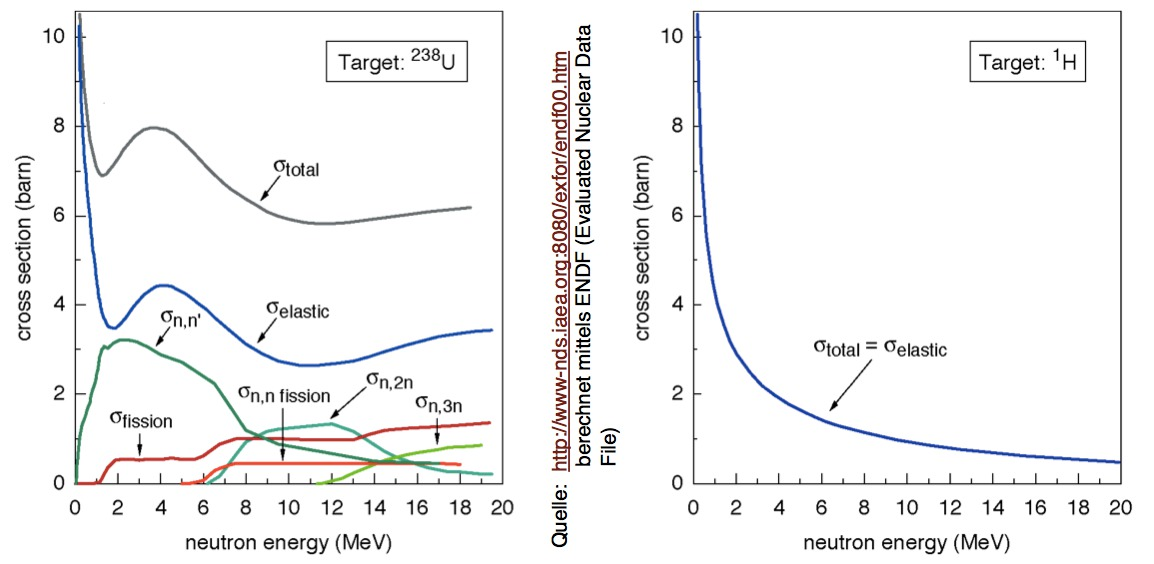
\includegraphics[width=\textwidth]{Fig-01-20.jpg}
	\caption{Hadronische Wirkungsquerschnitte für hochenegetische Neutronen in Uran bzw. Wasserstoff}
	\label{hadrwewi2}
\end{figure}

\begin{figure}[H]
	\centering
	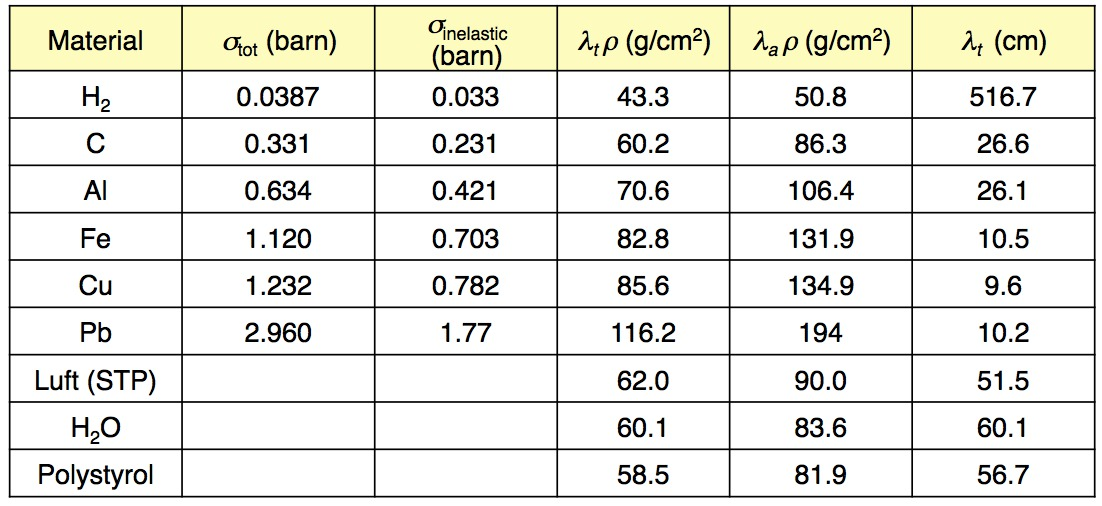
\includegraphics[width=\textwidth]{Fig-01-21.jpg}
	\caption{Wirkungsquerschnitte und Absorptionslängen für hochenergetische Neutronen ($\approx
	100\,$GeV) in diversen Materialien}
	\label{hadrwewitab}
\end{figure}